\documentclass[10pt]{article}
\usepackage[ngerman]{babel}
\usepackage[utf8]{inputenc}
\usepackage[T1]{fontenc}
\usepackage{amsmath}
\usepackage{amsfonts}
\usepackage{amssymb}
\usepackage[version=4]{mhchem}
\usepackage{stmaryrd}
\usepackage{graphicx}
\usepackage[export]{adjustbox}
\graphicspath{ {./images/} }

\title{Hauptprüfung Abiturprüfung 2022 - Leistungsfach }

\author{Alexander Schwarz\\
www.mathe-aufgaben.com}
\date{}


\begin{document}
\maketitle
 Baden-WürttembergJuni 2022

\section*{Aufgabe A 1.1 (13 VP)}
Die Abbildung zeigt den Graphen $G_{f}$ der Funktion $f$ mit\\
$f(x)=x^{3}-6 x^{2}+8 x$.\\
a) Berechnen Sie die Nullstellen von f. (1,5 VP) Berechnen Sie die Koordinaten des Wendepunktes W von $\mathrm{G}_{\mathrm{f}}$. (1,5 VP)

Die Gerade $t_{1}$ ist die Tangente an $G_{f}$ in $W$. Zeigen Sie, dass $y=-4 x+8$ eine Gleichung von $\mathrm{t}_{1}$ ist. (1 VP)\\
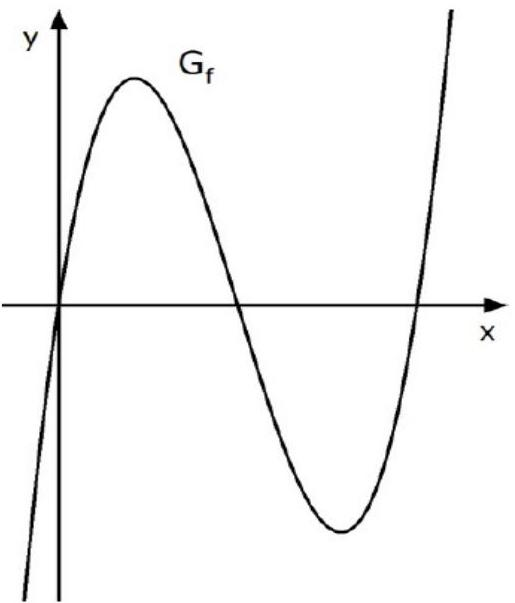
\includegraphics[max width=\textwidth, center]{2025_04_24_0a47e5696ee2d59b69d4g-2}\\
b) Die Gerade $t_{2}$ ist die Tangente an $G_{f}$ im Ursprung O. Die Geraden $t_{1}$ und $t_{2}$ schneiden sich im Punkt Q. Berechnen Sie für das Dreieck OWQ die Weite des Innenwinkels bei Q.

Für ein $u>0$ ist die Tangente an $G_{f}$ im Punkt $B(u \mid f(u))$ parallel zu $t_{2}$. Bestimmen Sie den Wert von u.\\
c) Die Funktion $I_{0}$ mit $I_{0}(x)=\int_{0}^{x} f(t) d t$ besitzt im Intervall $[0 ; 4]$ inren maximalen Wert an der Stelle $x_{0}$. Geben Sie $x_{0}$ an und begründen Sie Ihre Angabe. (1,5 VP)\\
d) Für die Funktion $h$ mit $h(x)=x^{3}-4 x$ gilt $f(x)=h(x-2)$. Erläutern Sie, welche Symmetrieeigenschaft daraus für $G_{f}$ folgt.\\
e) Der Graph $\mathrm{G}_{\mathrm{f}^{*}}$ entsteht durch Spiegelung des Graphen $\mathrm{G}_{\mathrm{f}}$ an der Geraden mit der Gleichung $x=a$. Die Tangente an $G_{f^{*}}$ im Wendepunkt von $G_{f^{*}}$ schneidet die $y$-Achse im Punkt S(0|16). Bestimmen Sie den Wert von a.\\
(2,5 VP)

\section*{Aufgabe A 1.2 (7 VP)}
Für jedes $\mathrm{a}>0$ ist die Funktion $\mathrm{f}_{\mathrm{a}}$ gegeben durch $\mathrm{f}_{\mathrm{a}}(\mathrm{x})=\mathrm{a} \cdot \sin (\mathrm{a} \cdot \pi \cdot \mathrm{x})$.\\
Die zugehörigen Graphen werden mit $\mathrm{G}_{\mathrm{a}}$ bezeichnet.\\
Der Punkt $H_{a}\left(\left.\frac{1}{2 a} \right\rvert\, a\right)$ ist ein Hochpunkt von $G_{a}$.\\
a) Geben Sie die Periode von $f_{a}$ an.

Der Punkt $\mathrm{H}_{\mathrm{a}}$ bildet mit den beiden von $\mathrm{H}_{\mathrm{a}}$ am wenigsten weit entfernten Tiefpunkten von $\mathrm{G}_{\mathrm{a}}$ ein Dreieck. Zeigen Sie, dass der Flächeninhalt dieses Dreiecks unabhängig von a ist.\\
b) Ermitteln Sie den Wert von a, für den $\mathrm{H}_{\mathrm{a}}$ vom Ursprung den Abstand 1 hat.\\
c) Bestimmen Sie eine Gleichung der Kurve K , auf der alle Punkte $\mathrm{H}_{\mathrm{a}}$ liegen.\\
(1 VP)\\
Auf K gibt es einen Punkt $\mathrm{H}_{\mathrm{a}}$, in dem die Tangente an K parallel zur Geraden mit der Gleichung $y=-2 x$ ist. Bestimmen Sie den Wert von a.\\
(1,5 VP)

\section*{Lösungen}
\section*{Aufgabe A 1.1}
a) Berechnen Sie die Nullstellen von f.

$$
f(x)=x^{3}-6 x^{2}+8 x
$$

Bedingung: $f(x)=0$\\
$x^{3}-6 x^{2}+8 x=0$\\
$\Leftrightarrow x \cdot\left(x^{2}-6 x+8\right)=0$ Lösung mit dem Satz vom Nullprodukt\\
I) $x_{1}=0$\\
II) $\mathrm{x}^{2}-6 \mathrm{x}+8=0 \Rightarrow \mathrm{x}_{2,3}=\frac{6 \pm \sqrt{36-32}}{2}=\frac{6 \pm 2}{2} \quad \mathrm{x}_{2}=4 \quad \mathrm{x}_{3}=2$

Berechnen Sie die Koordinaten des Wendepunktes $W$ von $G_{f}$.

$$
\begin{aligned}
& f^{\prime}(x)=3 x^{2}-12 x+8 \\
& f^{\prime \prime}(x)=6 x-12 \\
& f^{\prime \prime \prime}(x)=6
\end{aligned}
$$

Hinreichende Bedingung für den Wendepunkt: $f^{\prime \prime}(x)=0$ und $f^{\prime \prime \prime}(x) \neq 0$\\
$6 x-12=0 \Leftrightarrow x=2$\\
$\mathrm{f}^{\prime \prime}(2)=6 \neq 0$, damit existiert bei $\mathrm{x}=2$ eine Wendestelle\\
Wegen $f(2)=0$ ergibt sich als Wendepunkt $W(2 \mid 0)$.\\
Zeigen Sie, dass $\mathrm{y}=-4 \mathrm{x}+8$ eine Gleichung von $\mathrm{t}_{1}$ ist.\\
Ansatz für die Tangentengleichung an der Stelle $x=2: y=f^{\prime}(2) \cdot(x-2)+f(2)$ Es gilt $f^{\prime}(2)=3 \cdot 4-12 \cdot 2+8=-4$ und $f(2)=0$.

Gleichung der Tangente: $y=-4(x-2)+0 \Leftrightarrow y=-4 x+8$ was $z u$ zeigen war\\
b) Berechnen Sie für das Dreieck OWQ die Weite des Innenwinkels bei Q.

Zur Berechnung des Innenwinkels werden die Steigungen der beiden Tangenten benötigt.

Steigung von $t_{1}: m_{1}=-4$\\
Steigung von $t_{2}: m_{2}=f^{\prime}(0)=8$

Steigungswinkel der Tangente $t_{1}: \tan \left(\alpha_{1}\right)=-4 \Rightarrow \alpha_{1} \approx-76,0^{\circ}$\\
Steigungswinkel der Tangente $\mathrm{t}_{2}: \tan \left(\alpha_{2}\right)=8 \Rightarrow \alpha_{2} \approx 82,9^{\circ}$

Differenz der Steigungswinkel: $\alpha_{2}-\alpha_{1}=82,9^{\circ}-\left(-76,0^{\circ}\right)=158,9^{\circ}$\\
Somit ist $\alpha_{3}=180^{\circ}-158,9^{\circ}=21,1^{\circ}$ die Winkelweite bei $Q$.

Bestimmen Sie den Wert von u.\\
Bedingung: $\mathrm{f}^{\prime}(\mathrm{u})=8$\\
$3 u^{2}-12 u+8=8 \Leftrightarrow 3 u^{2}-12 u=0 \Leftrightarrow u(3 u-12)=0 \quad$ Satz vom Nullprodukt\\
I) $u=0$\\
II) $u=4$

Wegen $\mathrm{u}>0$ gilt $\mathrm{u}=4$.\\
c) Geben Sie $\mathrm{x}_{0}$ an und begründen Sie Ihre Angabe.

Die gesuchte Stelle ist $x_{0}=2$.\\
Begründung:\\
1.Möglichkeit:

Die Funktion $\mathrm{I}_{0}$ ist eine Integralfunktion von $f$ und damit eine spezielle\\
Stammfunktion von f. Die Maximumstelle findet sich an der Nullstelle von f, an der ein Vorzeichenwechsel von + nach - vorliegt. Dies ist bei $x=2$ der Fall (siehe Aufgabe a)).\\
2.Möglichkeit:

Die Funktion $\mathrm{I}_{0}$ beschreibt den orientierten Flächeninhalt zwischen dem Graphen von f und der x-Achse. Der Graph von f verläuft für $0<x<2$ oberhalb (Integralfunktion $I_{0}$ ist in diesem Intervall positiv) und für $2<x<4$ unterhalb der $x$-Achse (Integralfunktion $I_{0}$ ist in diesem Intervall negativ).\\
d) Erläutern Sie, welche Symmetrieeigenschaft daraus für $\mathrm{G}_{\mathrm{f}}$ folgt.

Der Graph $\mathrm{G}_{\mathrm{h}}$ von h ist punktsymmetrisch zum Ursprung, denn der\\
Funktionsterm von $h$ enthält nur Potenzen von x mit ungeraden Hochzahlen (Exponenten).\\
Das Schaubild $G_{f}$ von $f$ ist gegenüber $G_{h}$ um 2 Einheiten nach rechts verschoben. Daher ist $G_{f}$ punktsymmetrisch zu $W(2 \mid 0)$.\\
e) Bestimmen Sie den Wert von a.

Die Steigung der Wendetangente an das Schaubild von f ist $\mathrm{m}=-4$. Durch die Spiegelung des Schaubildes an der senkrechten Geraden x = a ändert sich die Steigung der Wendetangente $\mathrm{zu} \mathrm{m}^{*}=4$.\\
Da die Wendetangente an $\mathrm{G}_{\mathrm{f}^{*}}$ durch $\mathrm{S}(0 \mid 16)$ verläuft, ist die Gleichung der Wendetangente an $G_{f^{*}} y=4 x+16$.

Durch die Spiegelung an der Geraden $\mathrm{x}=$ a liegt der Wendepunkt $\mathrm{W}^{*}$ von $\mathrm{G}_{\mathrm{f}}{ }^{*}$ weiterhin auf der x-Achse.

Berechnung der Nullstelle der Wendentangente an $G_{f}: 0=4 x+16 \Leftrightarrow x=-4$ Daher ist $\mathrm{W}^{*}(-4 \mid 0)$ der Wendepunkt von $\mathrm{G}_{\mathrm{f}^{*}}$.

Der Wendepunkt von $G_{f}$ ist $W(2 \mid 0)$.\\
Um die Wendestelle von $x=2$ nach $x^{*}=-4$ zu bringen, muss der Punkt an der senkrechten Geraden $x=-1$ gespiegelt werden (Mittelwert von 2 und -4).\\
Daher ist $\mathrm{a}=\mathbf{- 1}$.

\section*{Aufgabe A 1.2}
a) Geben Sie die Periode von $\mathrm{f}_{\mathrm{a}}$ an.

Periode $\mathrm{p}=\frac{2 \pi}{\pi \cdot \mathrm{a}}=\frac{2}{\mathrm{a}}$\\
Zeigen Sie, dass der Flächeninhalt dieses Dreiecks unabhängig von a ist.

Skizze:\\
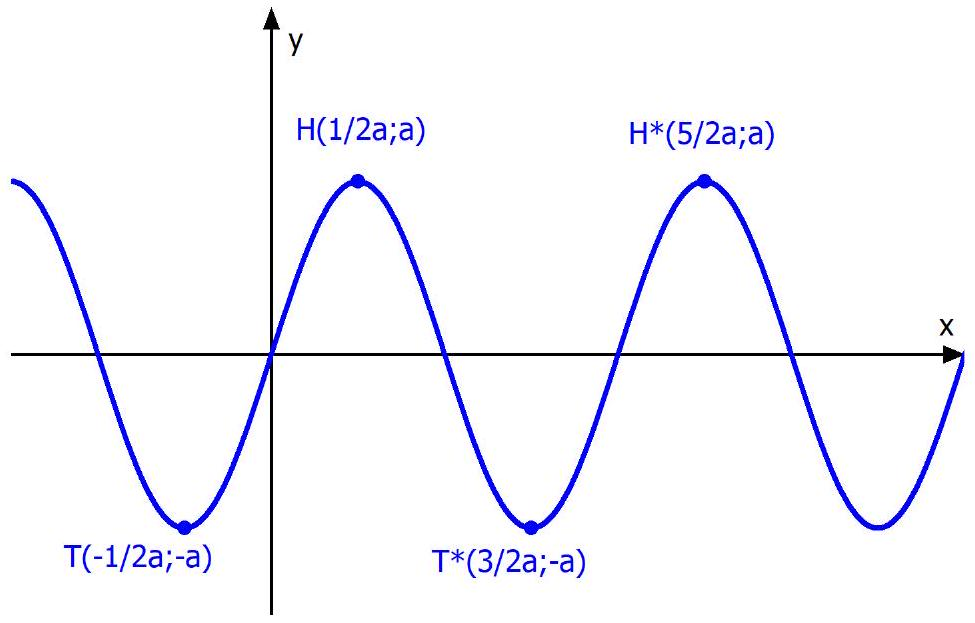
\includegraphics[max width=\textwidth, center]{2025_04_24_0a47e5696ee2d59b69d4g-6}

Gesucht ist der Flächeninhalt des Dreiecks T, T*, H.\\
$A_{\text {Dreieck }}=\frac{1}{2} \cdot \mathrm{~g} \cdot \mathrm{~h}=\frac{1}{2} \cdot \overline{\mathrm{TT}^{*}} \cdot \mathrm{~h}=\frac{1}{2} \cdot \frac{4}{2 \mathrm{a}} \cdot 2 \mathrm{a}=2$\\
Damit ist der Inhalt des Dreiecks unabhängig von a.\\
b) Abstand des Punktes $\mathrm{H}\left(\left.\frac{1}{2 \mathrm{a}} \right\rvert\, \mathrm{a}\right)$ vom Ursprung $\mathrm{O}(0 \mid 0)$ :\\
$\left.d\left(\mathrm{H}_{\mathrm{a}}, \mathrm{O}\right)=\sqrt{\left(\frac{1}{2 \mathrm{a}}\right)^{2}+\mathrm{a}^{2}}=1 \right\rvert\,$ quadrieren\\
$\left.\frac{1}{4 a^{2}}+a^{2}=1 \quad \right\rvert\, \cdot 4 a^{2}$\\
$1+4 a^{4}=4 a^{2}$\\
$\Leftrightarrow 4 a^{4}-4 a^{2}+1=0 \quad$ Substitution $a^{2}=u$\\
$4 u^{2}-4 u+1=0$\\
abc-Formel: $\quad u_{1,2}=\frac{4 \pm \sqrt{16-16}}{8}=\frac{4 \pm 0}{8}=\frac{1}{2}$\\
Rücksubstitution: $a^{2}=\frac{1}{2} \Rightarrow a=\sqrt{\frac{1}{2}} \quad($ da $a>0$ ist)\\
Probe, ob $a=\sqrt{\frac{1}{2}}$ eine Lösung der Wurzelgleichung ist:\\
$\sqrt{\left(\frac{1}{2 \cdot \sqrt{0,5}}\right)^{2}+\sqrt{0,5}^{2}}=1$ ist eine wahre Aussage.\\
Der gesuchte Wert ist $\mathrm{a}=\sqrt{\frac{1}{2}}$.\\
c) Bestimmen Sie eine Gleichung der Kurve K, auf der alle Punkte $\mathrm{H}_{\mathrm{a}}$ liegen.

Trennung der Koordinaten des Hochpunktes $\mathrm{H}_{\mathrm{a}}\left(\left.\frac{1}{2 \mathrm{a}} \right\rvert\, \mathrm{a}\right)$ :\\
$x=\frac{1}{2 \mathrm{a}}\left({ }^{*}\right)$ und $\mathrm{y}=\mathrm{a}\left({ }^{* *}\right)$\\
$\left(^{*}\right)$ nach a auflösen: $a=\frac{1}{2 x}$\\
Einsetzen in $\left(^{* *}\right)$ ergibt die Gleichung von $\mathrm{K}: \mathrm{y}=\frac{1}{2 \mathrm{x}}$ mit $\mathrm{x}>0($ wegen $\mathrm{a}>0$ ).

\section*{Bestimmen Sie den Wert von a.}
Gleichung der Ortskurve: $k(x)=\frac{1}{2 x}=\frac{1}{2} x^{-1}$ mit $k^{\prime}(x)=-\frac{1}{2} x^{-2}=-\frac{1}{2 x^{2}}$\\
Bedingung: $k^{\prime}(x)=-2: \quad-\frac{1}{2 x^{2}}=-2 \Leftrightarrow-1=-4 x^{2} \Leftrightarrow x^{2}=\frac{1}{4} \Rightarrow x_{1,2}= \pm \frac{1}{2}$\\
Für $\mathrm{x}_{1}=\frac{1}{2}$ gilt $\frac{1}{2 \mathrm{a}}=\frac{1}{2} \Leftrightarrow \mathrm{a}=1$\\
Für $\mathrm{x}_{2}=-\frac{1}{2}$ gilt $\frac{1}{2 \mathrm{a}}=-\frac{1}{2} \Leftrightarrow \mathrm{a}=-1$\\
Wegen $\mathrm{a}>0$ ist $\mathrm{a}=1$.


\end{document}